\documentclass[geometry-lectures-21.tex]{subfiles}
\begin{document}

\section{Symplectic geometry}


In this lecture, we will introduce symplectic geometry and learn the relation to classical mechanics. I highly recommend a great classic \cite{arnol1974mathematical} on this subject to you, and I guarantee that it is a wonderful-read. The relation between symplectic geometry and classical mechanics dates back to the work of Lagrange and Poisson in 1808 \cite{Lagrange1,Lagrange2,Poisson1,Poisson2}. Their works are formulated in a clear language, so-called Hamiltonian formalism \cite{hamilton1834general,hamilton1835second,Cauchy}, and it becomes deeper and deeper, involving dynamical systems, Lie groups, integrable systems and deformation quantizations in the 20th century. In the 1980s, the seminal works by Gromov \cite{gromov1985pseudo} and Floer \cite{floer1988instanton,floer1988morse,floer1989witten} open up a new area that studies symplectic manifolds globally, and it gives one aspect of ``quantum geometry''. Although Gauss-Bonnet theorem in Riemannian geometry and Riemann-Roch theorem in complex geometry preceded long before, we need more sophisticated techniques to study global topology in symplectic geometry simply because symplectic geometry is difficult. Hence, we just open the door to such a profound subject in this lecture.


\subsection{Hamiltonian formulation of classical mechanics}
Let us review Hamiltonian dynamical systems to connect symplectic geometry. The action of a point particle with mass $m$ move in a potential $V(q)$ is written as
$$
S=\int L(q,\dot{q}) d t~,\qquad L(q,\dot{q})=\frac12 m \dot{q}^2-V(q)~,
$$
where $q=\left(q_{1}, \ldots q_{n}\right)$ is a vector of $n$-dimensional space. Its Euler-Lagrange equation is described by the Newton equations
$$
m \ddot{q}_{i}=-\frac{\partial U}{\partial q_{i}}
$$
Introducing the momentum $p=\left(p_{1}, \ldots, p_{n}\right),$ where $p_{i}=m \dot{q}_{i}$, the Hamiltonian can be written as
$$
H=p\dot{q}-L=\frac{1}{2 m} p^{2}+V(q)
$$
The Hamiltonian is conserved
$$
\frac{d H}{d t}=\frac{1}{m} p_{i} \dot{p}_{i}+\dot{q}_{i} \frac{\partial U}{\partial q_{i}}=\frac{1}{m} m^{2} \dot{q}_{i} \ddot{q}_{i}+\dot{q}_{i} \frac{\partial U}{\partial q_{i}}=0
$$
due to the Newton equations of motion. Moreover, the equations of motion can be rewritten in Hamilton's canonical form
\be\label{Hamilton-eq}
\dot{q}_{j}=\frac{\partial H}{\partial p_{j}}~, \quad \dot{p}_{j}=-\frac{\partial H}{\partial q_{j}}~.
\ee
These can be understood as the Euler-Lagrange equation of the action
$$
S=\int({p} \cdot d {q}-H({q}, {p}) d t)~.
$$
Their importance lies in the fact that they are valid for arbitrary dependence of $H \equiv H(p, q)$ on the dynamical variables $p$ and $q$. To write it more elegant way, we consider the phase space $\bR^{2n}$ with coordinate $x=(p_1,\ldots,p_n,q_1,\ldots,q_n)$ with the gradient vector field $\textrm{grad} X=(\frac{\partial H}{\partial p_{j}}, \frac{\partial H}{\partial q_{j}} )$ of $H$. Using $2 n \times 2 n$ matrix
$$
J=\left(\begin{array}{rr}
0&-I_n\\I_n&0
\end{array}\right)~,
$$
the Hamilton's canonical equations of motion can be written in the form
$$
\dot{x}=J \cdot \nabla H, \quad \text { or } \quad J \cdot \dot{x}=-\nabla H
$$
This form of equations were written for the first time by Lagrange in 1808 \cite{Lagrange1}. Furthermore, we introduce the Poisson bracket
\be\label{Poisson}
\{f, g\}=J^{i j} \partial_{i}f \partial_{j} g=\sum_{j=1}^{n}\frac{\partial f}{\partial p_{j}} \frac{\partial g}{\partial q_{j}}-\frac{\partial f}{\partial q_{j}} \frac{\partial g}{\partial p_{j}}~.
\ee
The Hamiltonian equations can be now rephrased in the form
\be\label{Hamilton-eq2}
\dot{x}=\left\{H, x\right\} ~.
\ee
This is the birth of symplectic geometry!



\subsection{Symplectic manifolds}
A symplectic form on a smooth manifold $M$ is non-degenerate closed 2-form $\omega$. ``Non-degenerate'' means that the mapping $\omega : TM \to T^*M$; $X \mapsto \omega(X,-)$
 is an isomorphism. We denote the 1-form $\omega(X,-)$ by $i(X)\omega$.


 The couple ($M, \omega$) of a smooth manifold $M$ and a symplectic form $\omega$ is called a
\textbf{symplectic manifold}. Any symplectic manifold is even-dimensional and if $M$ is closed with dim($M) =
2n$, $\omega^n$ is a volume-form.

Therefore, very roughly speaking, symplectic geometry studies a geometry in which the ``area'' of a two-dimensional surface $\Sigma$ is defined. Since $d\omega=0$, the ``area'' $\int_\Sigma \omega$ of a closed surface $\Sigma$ does not change even if $\Sigma$ is continuously deformed.


 \bexample\label{symp-R2n}
 Let $(p_1,\ldots, p_n,q_1,\ldots, q_n)$ be the standard coordinate of $\R^{2n}$. Then,
 $$
\omega=\sum_{i=1}^n dp_i\wedge dq_i~
 $$
 is the symplectic form.
 \eexample

 A symplectic manifold $(M,\omega)$ is called \textbf{exact} if there exists one form $\theta$ such that $\omega=d\theta$ where $\theta$ is called \textbf{Liouville 1-form}. The vector field $Z$ dual to the Liouville 1-form with respect to $\omega$
 $$
 i(Z)\omega=\theta
 $$
 is called \textbf{Liouville vector field}.

 \bexample[cotangent bundle]\label{cotangent-symplectic}
 The most important example of exact symplectic manifolds is a cotangent bundle $M=T^*N$ of a smooth manifold $N$. Given a local coordinate $(q_1,\cdots,q_n)$, they induces the coordinate $(p_1,\cdots,p_n)$ on the fiber $T^*_qN$. Then, the Liouville 1-form is written in terms of the local coordinate of $T^*N$
$$
\theta=\sum_{i=1}^np_id q_i
$$
so that the symplectic form can be locally written as
$$
\omega=\sum_{i=1}^n dp_i\wedge dq_i~.
$$
 \eexample
%
 \bexample
The complex projective space
$$
\CP^n=\left(\mathbb{C}^{n+1} \backslash\{0\}\right) / \mathbb{C}^{\times}
$$
has a non-denerate 2-form called the \textbf{Fubini-Study form}
\bea
\omega_{\textrm{FS}}=&\sqrt{-1} \partial \bar{\partial} \log \left(\left|z_{1}\right|^{2}+\cdots+\left|z_{n+1}\right|^{2}\right)\cr
=&\sqrt{-1} \frac{\sum_{i=1}^{n+1} d z_{i} \wedge d \bar{z}_{i}-\left(\sum_{i=1}^{n+1} \bar{z}_{i} \wedge d z_{i}\right) \wedge\left(\sum_{i=1}^{n+1} z_{i} \wedge d \bar{z}_{i}\right)}{\left(\left|z_{1}\right|^{2}+\cdots+\left|z_{n+1}\right|^{2}\right)^{2}}
\eea
$(\CP^n,\omega_{\textrm{FS}})$ is a symplectic manifold, and moreorver it is a K\"ahler manifold.
 \eexample
%


 \bthm[Darboux's theorem]
Let $(M, \omega)$ be a $2n$-dimensional symplectic manifold,
and let $p$ be any point in $M$.
Then there is a coordinate chart $(U, q_1,\cdots , q_n,p_1,\cdots,p_n)$ centered at $p$ such that
on $U$
\be\label{symp}\omega=\sum_{i=1}^n dp_i\wedge dq_i~.\ee
 \ethm

This theorem states that any symplectic manifold is locally equivalent
to a Euclidean space with its standard symplectic structure. As a result, the most
important questions in symplectic geometry are the global ones.


\subsection*{Symplectomorphisms}

 The important maps in symplectic topology are the \textbf{symplectomorphisms}. A symplectomorphism
between two symplectic manifolds $(M, \omega_M)$ and $(N, \omega_N )$ is a diffeomorphism
$\psi : M\to N$ such that
$$
\psi^\ast \omega_N=\omega_M~.
$$
This condition is pretty strong. The necessary condition for the existence of symplectomorphisms is $\dim M \le\dim N$.

 \bexample[symplectic group]
Let $(\R^{2n},\omega)$ be as in Example \ref{symp-R2n}. Then, examples of symplectomorphisms are
$$
\Sp(n,\bR)=\{g\in GL(2n,\R) ~|g^TJg=J ~, \quad J=\begin{pmatrix}0&-I_n\\I_n&0\end{pmatrix}\}
$$
which is called the \textbf{symplectic group}.
 \eexample



 \bthm[Moser Stability Theorem] Let $(M, \omega_t)$ be a closed manifold with a family of
cohomologous symplectic forms. Then there is a family of symplectomorphisms $\psi_t
: M \to M$
such that
$$\psi_0 = 1~, \psi^*_t \omega_t = \omega_0~.$$
Moreover, if $\omega_t (q) = \omega_0 (q)$ for all points $q$ on a compact submanifold $Q$ of $M$, we may
assume $\psi_t$ is the identity on $Q$.
 \ethm


This theorem means that one cannot change the symplectic form in any important way by deforming it, provided that the cohomology class is unchanged.

 \subsection*{Lagrangian submanifolds}

 \bdefn[Lagrangian submanifold]
A Lagrangian submanifold of a symplectic manifold $(M,\omega )$ is a submanifold where the restriction of the symplectic form $\omega$ to $L\subset M$ is vanishing, i.e. $\omega |_{L}=0$ and ${\text{dim }}L=1/2\cdot {\text{dim }}M$.
\edefn

If we perturb a Lagrangian submanifold, then it is no longer Lagrangian in general. Thus, they are ``rigid'' objects in symplectic geometry. Since Lagrangian submanifolds play a significant role in symplectic geometry, Weinstein advertised the slogan that everything is a Lagrangian submanifold. (A. Weinstein's Lagrangian creed.)

 \bexample
The zero section $N$ of the cotangent bundle $M=T^*N$ is a Lagrangian submanifold. Let $f:Z\hookrightarrow N$ is an embedding. Then, the conormal bundle to $Z$ in $T^*N$ defined as
$$L_Z:=\{(x,\alpha)\in T^*N| x\in Z~, \quad \alpha(v)=0~ \textrm{for all}~ v\in T_xZ\}\subset T^*N~,$$
is a Lagrangian submanifold.
\eexample

It is known that the neighborhood of a Lagrangian also has the standard symplectic structure as its cotangent bundle.

 \bthm[Weinstein's tubular neighborhood theorem]
Every lagrangian submanifold $L$ in a symplectic manifold $(M,\omega)$ has a neighborhood $U$ which is symplectomorphic to  the cotangent bundle $T^*L$.
\ethm

 \subsection{Hamiltonian system}

 Any smooth function $H\in C^\infty(M)$ gives rise to a vector field $X_H$ defined uniquely
by the equation
$$i(X_H)\omega = -dH~,$$
where $i(X)\omega$ is the interior product in \eqref{interior}.
This vector field is called the \textbf{Hamiltonian vector field} with Hamiltonian $H$.
For $f,g\in C^\infty(M)$, we define the Poisson bracket by
$$
\{ f,g\}=\omega(X_f,X_g)=-X_f(g)=X_g(f)~.
$$


In the phase space $(\bR^{2n},\omega)$ of Example \ref{symp-R2n},
 the Poisson bracket of $f,g\in C^\infty(M)$ is expressed as \eqref{Poisson}. ALso, the flow of the Hamiltonian vector field $X_H$ associated to a Hamiltonian $H$ can be described by
 the Hamilton's canonical equations \eqref{Hamilton-eq} and \eqref{Hamilton-eq2}.

The Poisson bracket  satisfies the following properties
 \begin{description}
\item{Skew symmetry:} $ \{f,g\}=-\{g,f\}.$
\item{Jacobi identity:} $ \{f,\{g,h\}\}+\{g,\{h,f\}\}+\{h,\{f,g\}\}=0.$
\item{Leibniz's Rule:} $ \{fg,h\}=f\{g,h\}+g\{f,h\}.$
\end{description}
Using these properties, one can show that
$$
[X_f,X_g]=X_{\{f,g\}}~.
$$
 For $f\in C^\infty(M)$, the differentiation with respect to the Hamiltonian flow can be expressed by
 $$
 \frac{df}{dt}=\{H,f\}~.
 $$
If $\{f,H\}=0$, the flow $\varphi_s$ generated by $X_f$ is the symmetry of the Hamiltonian system with $H$. Namely, we have
$$
\frac{dH}{ds}=\{H,f\}=0~,
$$
 or equivalently,
 $$
 \frac{df}{dt}=\{H,f\}=0~.
 $$
This is called \textbf{Noether theorem}.


\bexample
If the system has spherical symmetry, the potential $V(r)$ is independent of $\theta$ and $\phi$. Then, the momenta $p_\theta$ and $p_\phi$ are conserved.
\eexample




 \subsection{Arnold-Liouville theorem}
Let us consider Poisson commuting functions (Hamiltonians)
$H_1, \cdots , H_k$ with $\{H_i, H_j\} = 0$ for all $i, j$. To insure that we are not discussing a degenerate situation, we assume that
$dH_1\wedge \cdots \wedge dH_k(x) \neq 0$ for $\forall x\in M$, in which $H_i$ are called \textbf{analytically independent}. Then, the maximal number of Poisson commuting functions is a half of dimension of $M$ which is $n$. A $2n$-dimensional symplectic manifold $(M,\omega)$ with $n$ Poisson commuting Hamiltonians is called \textbf{completely integrable system}.


\bthm[Arnold-Liouville theorem]
Let $H_1, \cdots , H_n$ be a completely integrable system on a $2n$-dimensional symplectic manifold $(M,\omega)$. Namely,
$\pi=(H_1, \cdots , H_n):M\to \R^n$ are analytically independent Poisson commuting functions with $\{H_i, H_j\} = 0$ for all $i, j$. Then, a compact connected component of the preimage of a non-singular point of $\pi$ is a Lagrangian submanifold that is diffeomorphic to a torus $T^n$.
\ethm

Let us denote the image of $\pi$ by $B$. Then, (compact connected component of) the preimage $L=\pi^{-1}(b)$ of $b\in B$ is diffeomorphic to $T^n$ so that we can take the angle coordinate
$$
(\phi_1\cdots \phi_n):	L\to T^n
$$
We can further take local coordinate $(I_1,\cdots,I_n)$ of $B$ that the symplectic form can be locally expressed as
$$
\omega=\sum_{i=1}^n dI_i\wedge  d\phi_i~,
$$
where $(\phi_i,I_i)$ are called \textbf{angle-action} coordinate.


\bexample
Let us consider the harmonic oscillator with Hamiltonian
 \[
  H(q, p) = \frac{1}{2}p^2 + \frac{1}{2}\omega^2 q^2~,
 \]
as an example. Since it is a 2-dimensional system, we only need a single integral. Since $H$ is a first integral for trivial reasons, this is an integrable Hamiltonian system.

 We can actually draw the lines on which $H$ is constant --- they are just ellipses:
 \begin{center}
  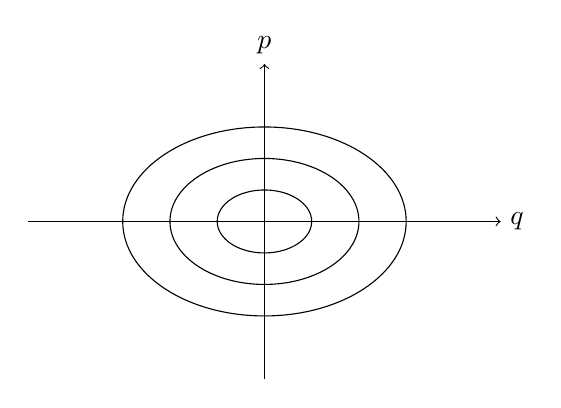
\begin{tikzpicture}
   \draw [->] (-3, 0) -- (3, 0) node [right] {$q$};
   \draw [->] (0, -2) -- (0, 2) node [above] {$p$};

   \foreach \x in {0.4, 0.8, 1.2} {
    \begin{scope}[scale=\x]
     \draw ellipse (1.5 and 1);
    \end{scope}
   }
  \end{tikzpicture}
 \end{center}
 We note that the ellipses are each homeomorphic to $S^1$. Now we introduce the coordinate transformation $(q, p) \mapsto (\phi, I)$, defined by
 \[
  q = \sqrt{\frac{2I}{\omega}} \sin \phi,\quad p = \sqrt{2I\omega} \cos \phi,
 \]
Hence, $\phi$ is the angle coordinate that parametrizes $S^1$ in the Arnold-Liouville theorem.

 We can manually show that this transformation is canonical. However, it is merely a computation, and we will not waste time doing that. In these new coordinates, the Hamiltonian looks like
 \[
  \tilde{H}(\phi, I) = H(q(\phi, I), p(\phi, I)) = \omega I~.
 \]
The Hamiltonian is independent of $\phi$! Therefore, the Hamilton equations become
 \[
  \dot\phi =- \frac{\partial \tilde{H}}{ \partial I} = \omega~,\qquad \dot{I} = \frac{\partial \tilde{H}}{\partial \phi} = 0~,
 \]
yielding
 \[
  \phi(t) = \phi_0 - \omega t~,\quad I(t) = I_0~.
 \]
It is interesting to consider the integral of the Liouville 1-form along a path of constant $H$:
 \begin{align*}
  \frac{1}{2\pi}\oint p \;\d q &= \frac{1}{2\pi} \int_0^{2\pi}p(\phi, I) \left(\frac{\partial q}{\partial \phi} \;\d \phi + \frac{\partial q}{\partial I} \;\d I\right)\\
  &= \frac{1}{2\pi} \int_0^{2\pi}p(\phi, I) \left(\frac{\partial q}{\partial \phi} \;\d \phi\right)\\
  &= \frac{1}{2\pi} \int_0^{2\pi} \sqrt{\frac{2I}{\omega}}\sqrt{2I\omega} \cos^2 \phi \;\d \phi\\
  &= I~.
 \end{align*}
We can always perform the integral of the Liouville 1-form along paths of constant $H$ without knowing anything about $I$ and $\phi$, which magically gives us the new coordinate $I$. This is the reason why it is called \textbf{integrable system}.
\eexample





\end{document}
